\section{Supervisión de servidor de impresión (SNMP)}

\subsubsection{Configuracion}

El proceso de configuracion será aplicado a una distribucion CentOS, el servicio de impresion con el cual se ejemplifica el documento es: CUPS.
Se inicia el sistema con las credenciales de super usuario root, con la restriccion de tener internet introducimos el comando:
\\
\begin{center}
\textbf{yum -y install cups}
\end {center}
						
\FloatBarrier
\begin{figure}[htbp!]
		\centering
			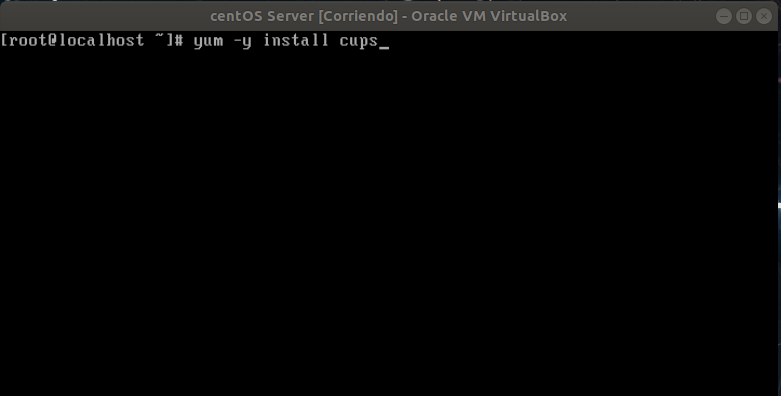
\includegraphics[width=.8 \textwidth]{images/r1}
		\caption{Comandos para la instalación de cups.}
		\label{image:r1}
\end{figure}
\FloatBarrier

Con lo cual habremos instalado todo lo necesario para iniciar el servicio de impresion cups, posteriormente debemos cambiar el archivo de configuracion por dos razones, la primera de ellas es para poner a la escucha el servidor y que otra pc pueda conectarse, el segundo motivo es para permitir que nuestra pc que ocupamos para el desarrollo pueda utilizar el servicio web que ofrece cups, ya que al tener una pc sin ambiente grafico, no es posible ver el servidor web. Para lograr lo anterior primeramente de forma opcional iniciamos una sesion ssh para conectarnos de forma remota y no tener que cambiar constantemente de equipo, para ello desde nuestra pc de desarrollo introducimos el comando:
\\
\begin{center}
\textbf{ssh root@direccion ip servidor}
\textbf{ej. ssh root@10.100.76.245}
\end {center}
\FloatBarrier
\begin{figure}[htbp!]
		\centering
			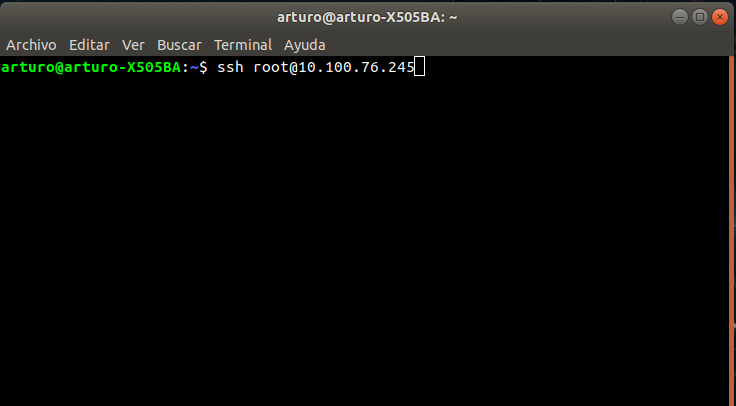
\includegraphics[width=.9\textwidth]{images/r2}
		\caption{Comandos para cambiar archivos de configuración.}
		\label{image:r2}
\end{figure}
\FloatBarrier

Posteriormente introducimos la contraseña y ya podemos trabajar en nuestra pc.
El siguiente paso es acceder al directorio de archivos de cups:
\\
\begin{center}
						\textbf{cd /etc/cups}
\end {center}
\FloatBarrier
\begin{figure}[htbp!]
		\centering
			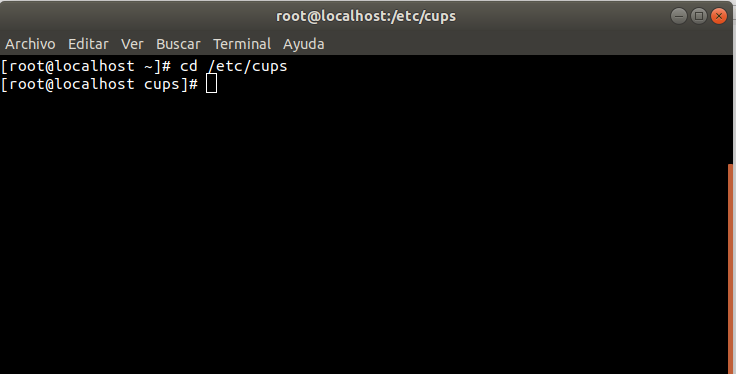
\includegraphics[width=.9\textwidth]{images/r3}
		\caption{Comandos para acceder al directorio de archivos.}
		\label{image:r3}
\end{figure}
\FloatBarrier
Abrimos el archivo de configuracion cupsd.conf
\\
\begin{center}
\textbf{vi cupsd.conf}
\end {center}
\FloatBarrier
\begin{figure}[htbp!]
		\centering
			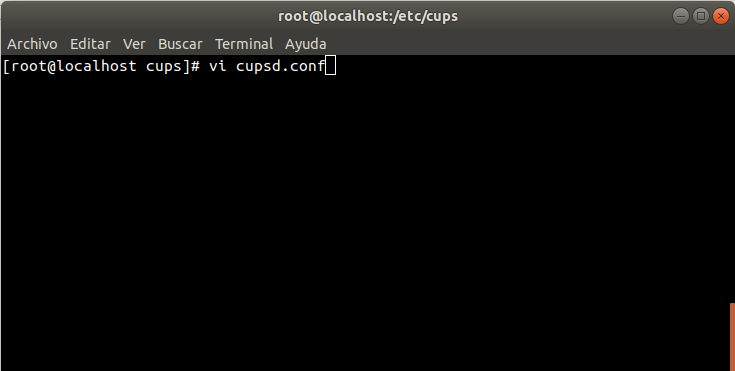
\includegraphics[width=.9\textwidth]{images/r4}
		\caption{Comandos.}
		\label{image:r4}
\end{figure}
\FloatBarrier
Agregamos una linea LISTEN para poner a la escucha nuestro servidor instroduciendo como parametro la direccion ip del servidor que tiene instalado el servicio de impresiones, indicando el puerto por defecto del servicio de impresion que es el 631.
\\
\begin{center}
					\textbf{LISTEN ip servidor:631}
					\textbf{ej. LISTEN 10.100.76.245:631}
\end {center}
\FloatBarrier
\begin{figure}[htbp!]
		\centering
			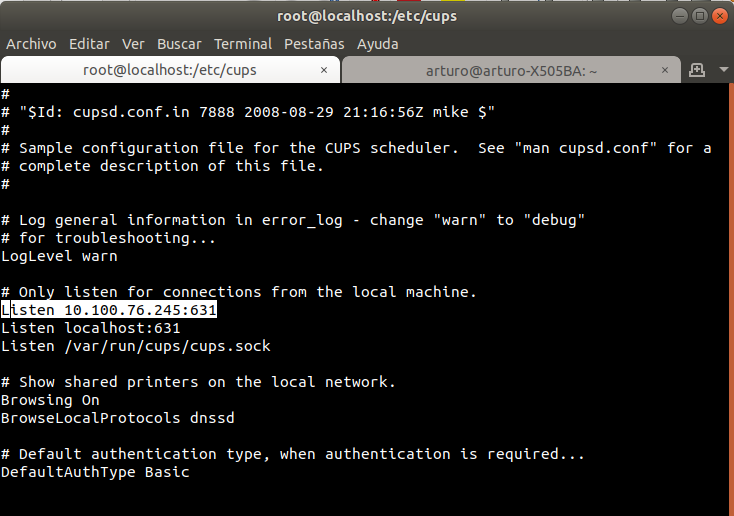
\includegraphics[width=.9\textwidth]{images/r5}
		\caption{Configuración del archivo cupsd.conf}
		\label{image:r}
\end{figure}
\FloatBarrier
Posteriormente agregamos tres lineas mas que implican el permiso a cierta direccion ip para que pueda utilizar o acceder al servicio y configuracion, lo logramos introduciendo una intruccion Allow seguido de la direccion ip de la pc de desarrollo
\\
\begin{center}
						\textbf{Allow ip pc desarrollo}
						\textbf{ej. Allow 10.100.69.24}
\end {center}
\FloatBarrier
\begin{figure}[htbp!]
		\centering
			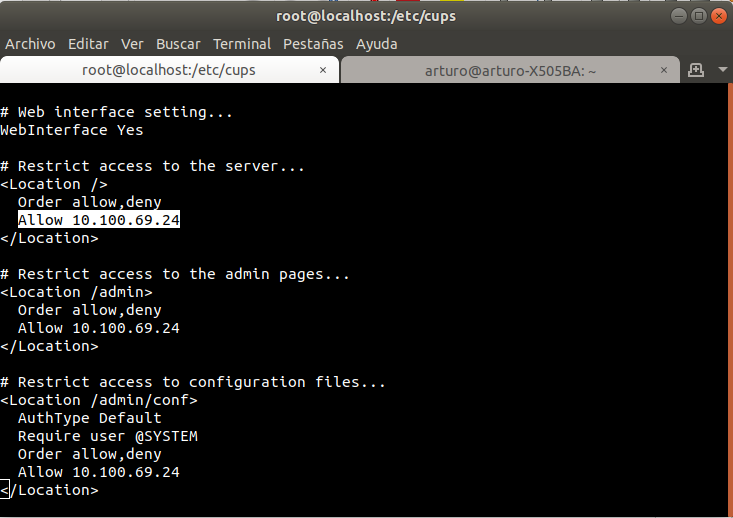
\includegraphics[width=.9\textwidth]{images/r6_1}
		\caption{Configuracion de la ip de la pc location}
		\label{image:r6_1}
\end{figure}
\FloatBarrier

\FloatBarrier
\begin{figure}[htbp!]
		\centering
			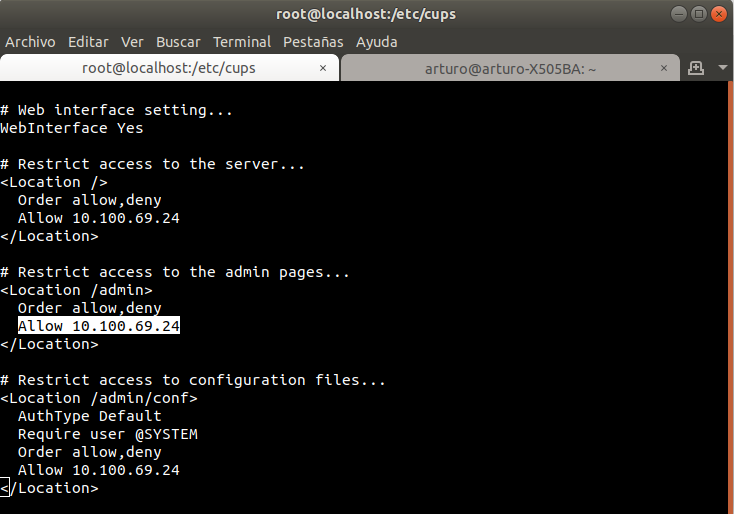
\includegraphics[width=.9\textwidth]{images/r6_2}
		\caption{Configuracion de la ip de la pc admin}
		\label{image:r6_2}
\end{figure}
\FloatBarrier

\FloatBarrier
\begin{figure}[htbp!]
		\centering
			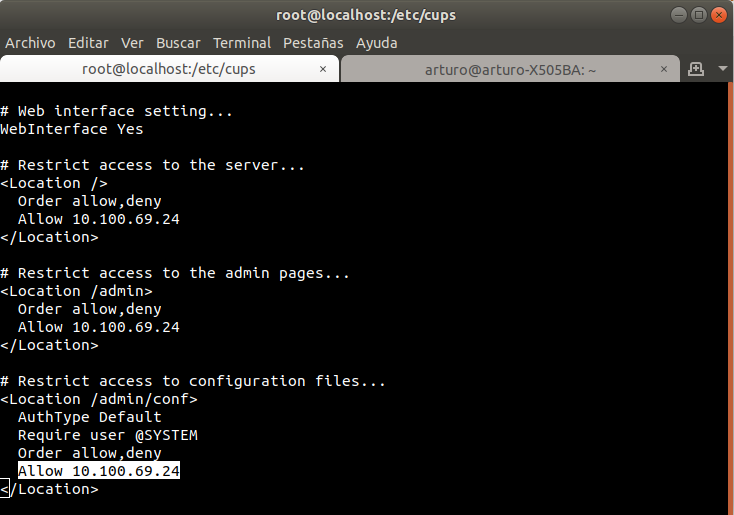
\includegraphics[width=.9\textwidth]{images/r6_3}
		\caption{Configuracion de la ip de la pc admin/conf}
		\label{image:r6_3}
\end{figure}
\FloatBarrier
Guardamos el archivo,  reiniciamos el servicio de impresion y apagamos el firewall.
\\
\begin{center}
						\textbf{systemctl restart cups}
						\textbf{systemctl stop firewalld}
\end {center}
\FloatBarrier
\begin{figure}[htbp!]
		\centering
			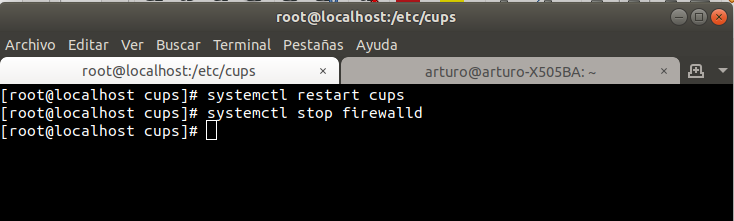
\includegraphics[width=.9\textwidth]{images/r7}
		\caption{Reinicio y apago de firewall}
		\label{image:r7}
\end{figure}
\FloatBarrier

Ahora probamos el servicio en nuestra pc de desarrollo introduciendo en un navegador la ip del servidor y el puerto. Con esto hemos completado la configura:
\\
\begin{center}
					\textbf{ej. http://192.168.100.12:631}
\end {center}
\FloatBarrier
\begin{figure}[htbp!]
		\centering
			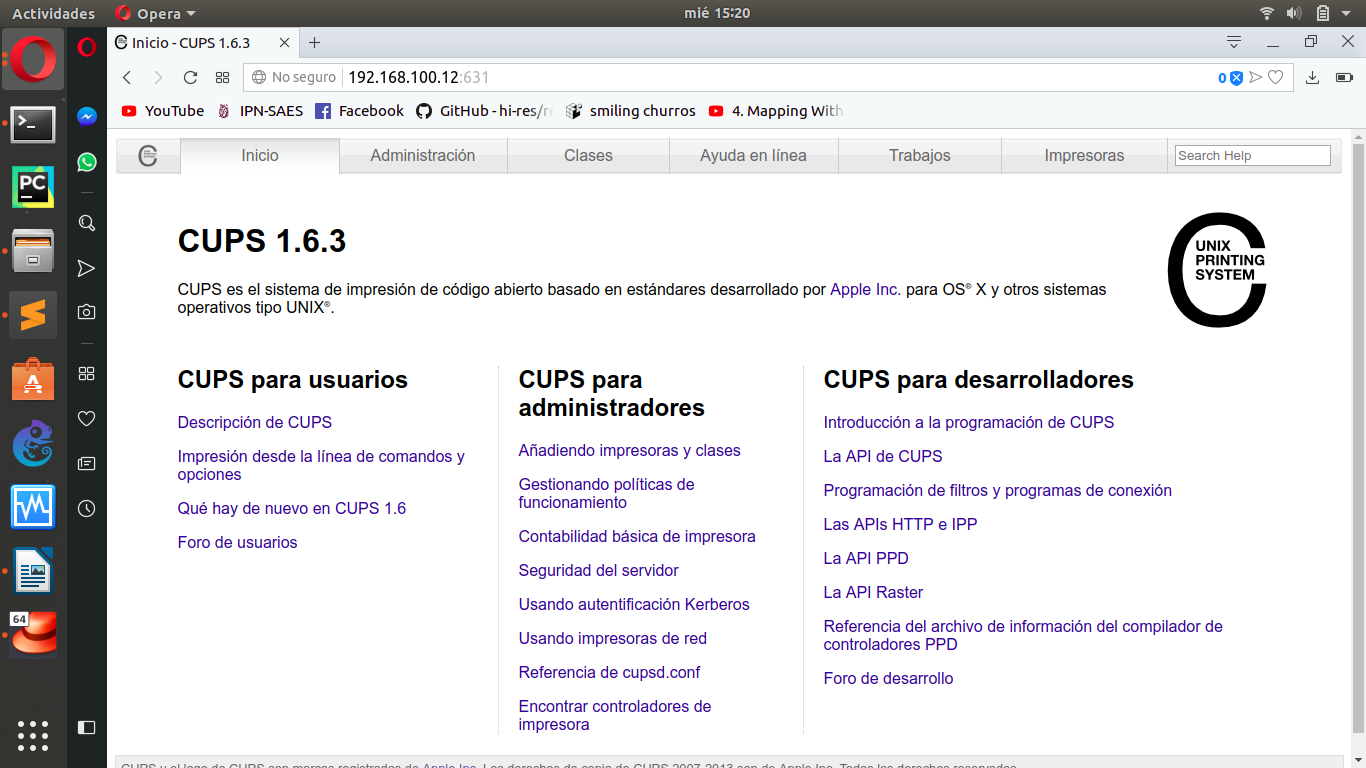
\includegraphics[width=.9\textwidth]{images/r8}
		\caption{Servicio activo}
		\label{image:r8}
\end{figure}
\FloatBarrier


\subsubsection{Monitorizacion de impresoras}

Anexamos las capturas de pantalla del codigo generado, con una nota extra, de que no contabamos con impresoras con tarjeta de red por lo que no fue posible obtener su informacion via snmp, posteriormente se explica cómo se solucionó el problema mediante ssh.
\\
La funcion \textbf{monitorear} en la linea 46 \ref{image:s2} tiene todo el procedimientos de tres aspectos fundamentales que son laconexion, la captura de datos y finalmente el tratamiento de la informacion para ser mostrada.
\\
La funcion \textbf{sshHilo} dentro de monitorear \ref{image:s6}, que podemos encontrar en la linea 181, establecemos una conexión ssh al servidor que cuenta con el servicio de impresionmediante la \textbf{librería pexpect}, introducimos las credenciales de inicio de sesion, lo mas importante recae en la linea 188, en donde se ejecuta el comando \textbf{lpstat -l -t} que nos junta la informacion de las impresoras que tiene conectadas, posteriormente cerramos esa sesion y abrimos un archivo llamado impresoras.txt donde se almacena la informacion obtenida del comando \textbf{lpstat}.
\\
La evaluacion del if en la linea 51 \ref{image:s2} nos indica si hubo un problema en la conexiony nos muestra una ventana de error.
De otro modo la funcion \textbf{establecer info} nos retorna un indicador si es que el servicio de impresion tiene conectada alguna impresora, en caso de no encontrar, nos muestra otra  entana indicando que no tiene impresoras por el momento.
\\
Finalmente al pasar por estos filtros se organiza la informacion para tener cierto formato y el usuario pueda obtener el estado de las impresoras.

\FloatBarrier
\begin{figure}[htbp!]
		\centering
			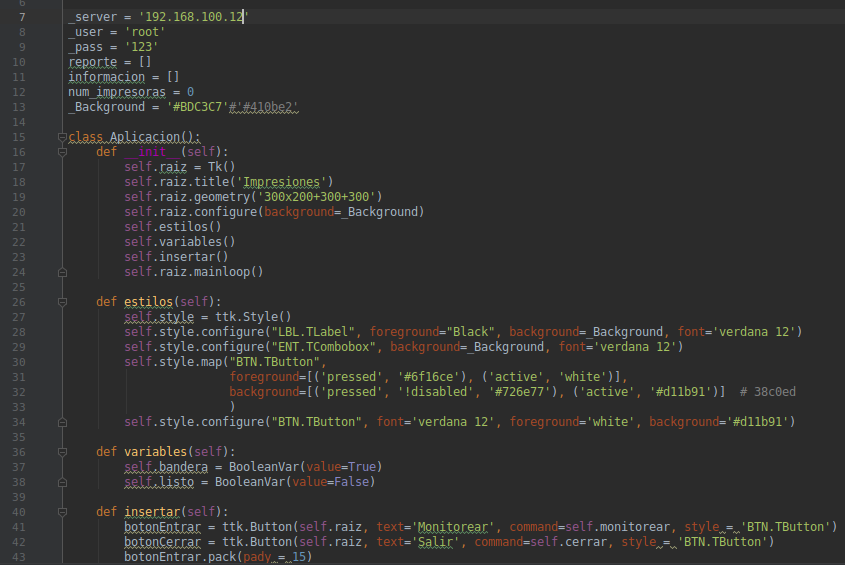
\includegraphics[width=.9\textwidth]{images/s1}
		\caption{Inicio del módulo de servicio de impresión}
		\label{image:s1}
\end{figure}
\FloatBarrier

\FloatBarrier
\begin{figure}[htbp!]
		\centering
			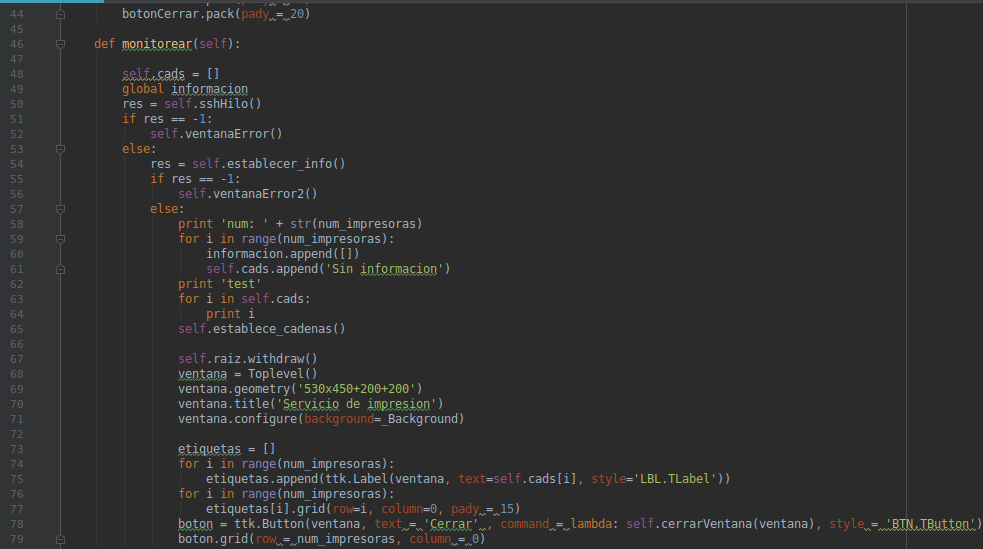
\includegraphics[width=.9\textwidth]{images/s2}
		\caption{Función monitoriar}
		\label{image:s2}
\end{figure}
\FloatBarrier

\FloatBarrier
\begin{figure}[htbp!]
		\centering
			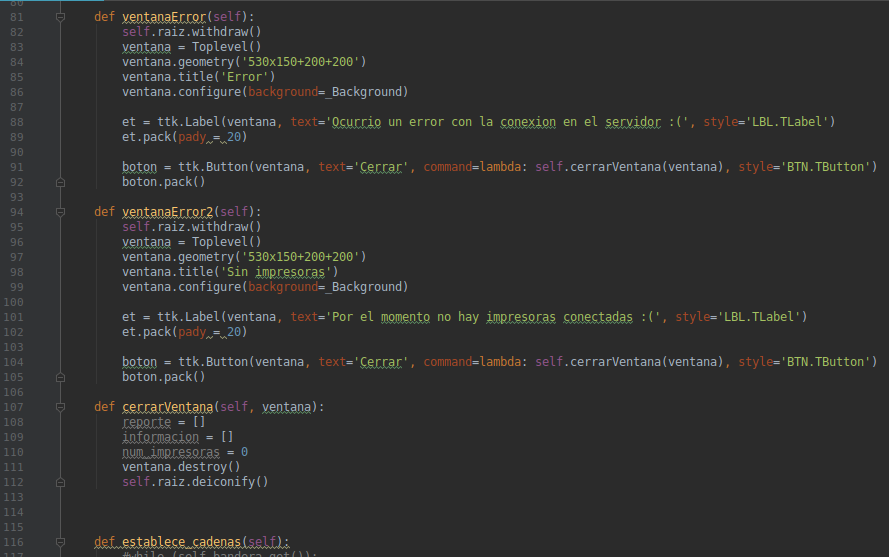
\includegraphics[width=.9\textwidth]{images/s3}
		\caption{Funciones de mensaje de error}
		\label{image:s3}
\end{figure}
\FloatBarrier

\FloatBarrier
\begin{figure}[htbp!]
		\centering
			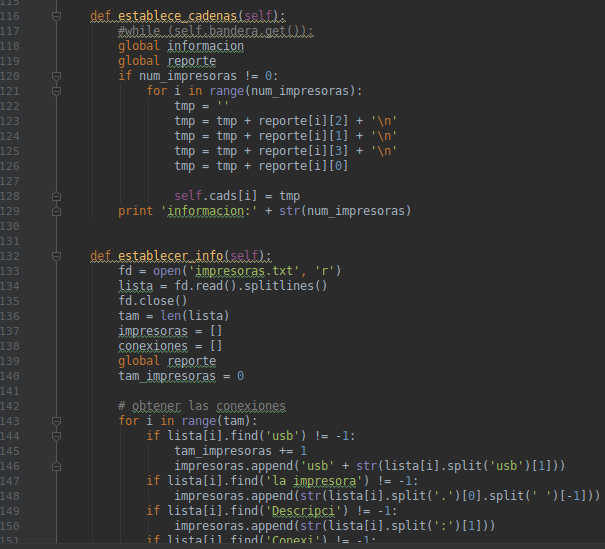
\includegraphics[width=.9\textwidth]{images/s4}
		\caption{Función Establecer Cadenas e info }
		\label{image:s4}
\end{figure}
\FloatBarrier

\FloatBarrier
\begin{figure}[htbp!]
		\centering
			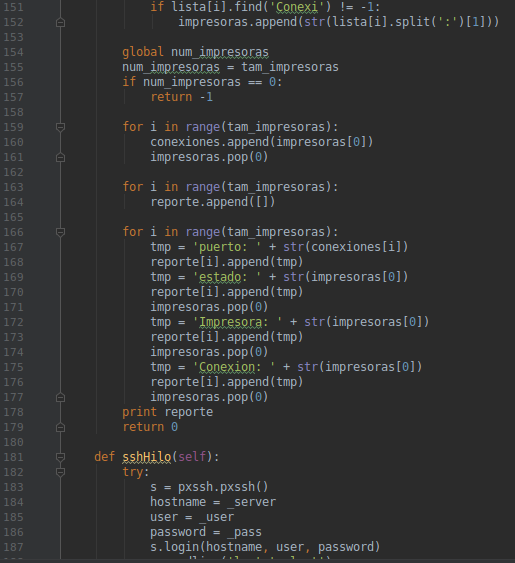
\includegraphics[width=.9\textwidth]{images/s5}
		\caption{Parametros que muestra una impresora activa}
		\label{image:s5}
\end{figure}
\FloatBarrier

\FloatBarrier
\begin{figure}[htbp!]
		\centering
			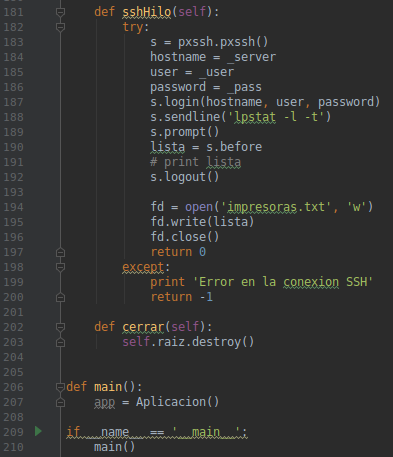
\includegraphics[width=.9\textwidth]{images/s6}
		\caption{funcion sshHilo}
		\label{image:s6}
\end{figure}
\FloatBarrier




\subsubsection{Funcionamiento}

Primero nos encontramos con un pequeño menú
\FloatBarrier
\begin{figure}[htbp!]
		\centering
			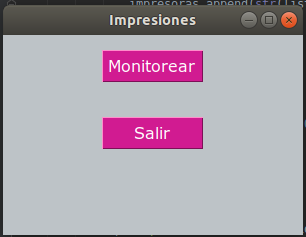
\includegraphics[width=.9\textwidth]{images/s7}
		\caption{Menú}
		\label{image:s7}
\end{figure}
\FloatBarrier

Dado caso que el servidor no se encunetre activo se manda un mensaje de alerta.
\FloatBarrier
\begin{figure}[htbp!]
		\centering
			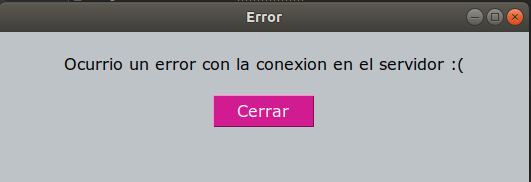
\includegraphics[width=.9\textwidth]{images/s8}
		\caption{Sin servidor}
		\label{image:s8}
\end{figure}
\FloatBarrier

De igual manera si no se encuentra una impresora se mostrara el siguiente mensaje \ref{image:s9}
\FloatBarrier
\begin{figure}[htbp!]
		\centering
			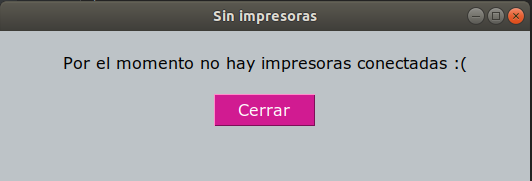
\includegraphics[width=.9\textwidth]{images/s9}
		\caption{Sin impresora}
		\label{image:s9}
\end{figure}
\FloatBarrier

Cuando se tiene el servidor corriendo y las impresoras conectadas nos mostrará la siguiente información que es el nombre de la impresora, su estado, conexion y en este caso el puerto. \ref{image:final} 

\FloatBarrier
\begin{figure}[htbp!]
		\centering
			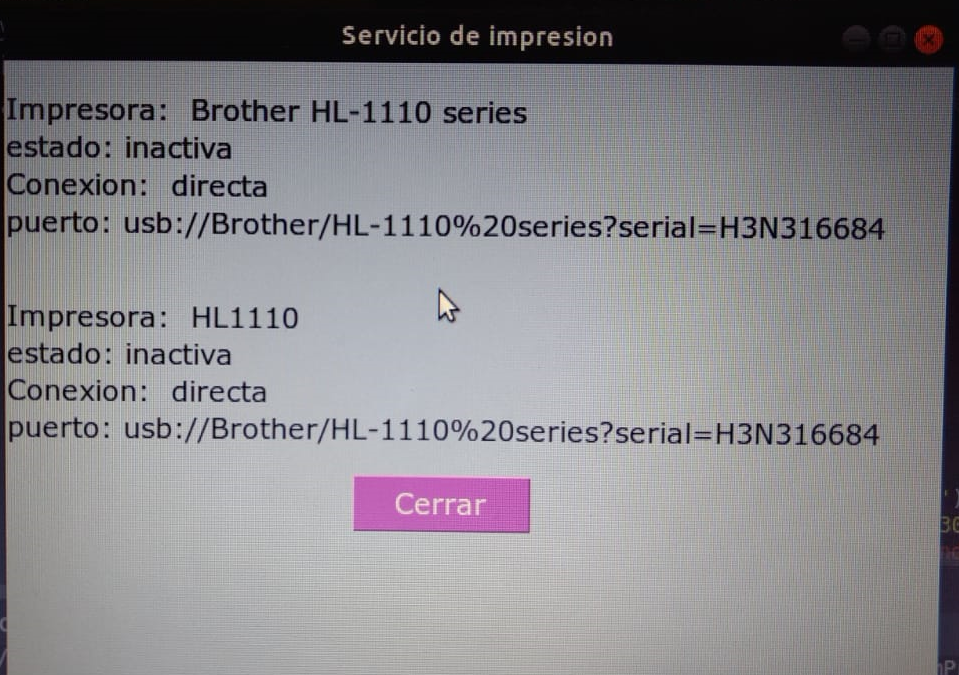
\includegraphics[width=.9\textwidth]{images/final}
		\caption{Impresoras conectadas}
		\label{image:final}
\end{figure}
\FloatBarrier